
\chapter{Integralrechnung}

Die eindimensionale Integralrechnung beschäftigt sich -- zumindest im sogenannten \emph{bestimmten} Fall -- mit der Messung von Flächeninhalten. Und zwar mit dem Maß der Fläche unter einer bestimmten Funktion. Das bedeutet, wir möchten mithilfe der Integralrechnung die Größe der Fläche bestimmen, die zwischen der $x$-Achse und einer Funktion $f(x)$ aufgespannt wird. Dafür begrenzen wir die Fläche, die uns interessiert, an der linken und rechten Seite durch ein Interval $[a,b]$. Allgemein gilt $a<b$. 

Im \emph{unbestimmten} Fall analysieren wir die Menge aller Flächeninhalte, wenn die Grenzen $a$ und $b$ nicht festgelegt sind. Vorweg sei erwähnt, dass man dadurch eine Funktion definieren kann, die -- falls man ihre Funktionswerte an den Stellen $a$ und $b$ auswertet -- unmittelbare Aussagen über den Flächeninhalt unter der Funktion $f$ gibt. Diese "`Flächeninhalts"'-Funktion wird einen interessanten Zusammenhang mit der Funktion $f$ haben. Und diesen Zusammenhang bezeichnet man gemeinhin als den \emph{Hauptsatz der Integral- und Differentialrechnung}, doch dazu später.  Sehen wir uns zur Illustration Abbildung \ref{fig:int1} an:

\begin{figure}[h!]
\centering
\begin{tikzpicture}[domain=0.25:2.75,scale=2]
%\draw[step=.5cm,lightgray,very thin] (-0.4,-0.4) grid (3.1,1.4);
\draw (-0.5,0) -- (3.1,0);
\draw (0,-0.5) -- (0,1.5);

\draw[gray,very thin](0.25,0.2474) -- (0.25,0)  node[below]{$a$} ;
\draw[gray,very thin](2.75,0.38166) -- (2.75,0)  node[below]{$b$} ;

\draw[color=black,thick]   plot[smooth] (\x,{sin(\x r)});

\node at (pi/2,0.4) {Fläche $F$};
\end{tikzpicture}
\caption{Das bestimmte Integral}
\label{fig:int1}
\end{figure}
Wir haben damit eine Fläche $F$ definiert, die an den Seiten und der Unterseite grade Ränder besitzt, aber an der Oberseite von der Funktion $f$ begrenzt wird. Wir kennen zwar die Funktion $f$, doch ist es uns nicht möglich, die Größe der Fläche unter dem Graph durch eine einfache Formel anzugeben. 

\section{Riemann-Integral}

Bernhard Riemann\footnote{\textbf{Georg Friedrich Bernhard Riemann} *17. September 1826 in Breselenz; \ding{61}20. Juli 1866 in Selasca} 

\subsection{Intervall Zerlegung}

\begin{definition}[Intervall Zerlegung]\index{Intervall Zerlegung}\index{Zerlegung}\label{def:zerlegung}
Zunächst wollen wir das Intervall $[a,b]$ in kleinere Teile zerlegen. Wir wählen uns dafür eine Menge von Punkten innerhalb dieses Intervalls und zwar auf folgende Weise:

\begin{enumerate}
\item Wir wählen $N+1$ Werte $x_i$ mit $0\le i \le N$.
\item Für alle $i$ gilt $a\le x_i \le b$.
\item Weiter sind die Ränder definiert als $x_0=a$ und $x_N=b$ und
\item $x_i < x_{i+1}$ für alle $0\le i < N$.
\end{enumerate}
Forderung 2 ist im Grunde unnötig, da mit 3 und 4 dies automatisch folgt. Aber der Klarheit halber nehmen wir diese Anforderung mit auf. Weiter definieren wir uns auf diese Weise $N$ Intervalle:

\begin{equation}
I_i = [x_{i-1},x_{i}], \text{ mit } i=1, \dots , N
\end{equation}
\end{definition}

Eine solche Aufteilung des Intervalls $[a,b]$ in diese kleineren Intervalle $[x_i,x_{i+1}]$ nennt man eine \emph{Intervall Zerlegung}. Wir haben keine weiteren Anforderungen an die $x_i$ Werte gestellt, als dass sie in einer Reihenfolge zwischen $a$ und $b$ liegen sollen. Die Abstände zwischen diesen Werten ist aber frei wählbar. Man könnte natürlich der Einfachheit halber sie \emph{äquidistant} wählen, also in einem gleichmäßigen Abstand. Doch das hat keinen Einfluss auf die späteren Berechnungen. 

\begin{definition}
Zu jedem dieser $N$ Intervalle wählen wir uns nun auch noch eine sogenannte \emph{Stützstelle} $s_i$ mit $i=1, \dots , N$. Diese liegt innerhalb des zugehörigen Intervalls:
\begin{equation}
s_i \in [x_{i-1},x_{i}]
\end{equation}
Eine solche Zerlegung wird mit $Z$ bezeichnet.
\end{definition}

Aber auch hier legen wir keine weiteren Anforderungen an $s_i$ fest, diese Stützstelle kann irgendwo in ihrem zugehörigen Intervall liegen.

\subsection{Riemann-Summe}\index{Riemann-Summe}

Zu jeder der im vorher genannten Stützstellen berechnen wir den Funktionswert von $f$  und multiplizieren ihn mit der breite des zugehörigen Intervalls.

\begin{equation}
F_i = f(s_i)\cdot (x_{i}-x_{i-1})
\end{equation}
Die Summe über diese Werte ist eine erste Annäherung an den Flächeninhalt $F$:

\begin{equation}
\sum_{i=1}^{N} F_i = \sum_{i=1}^{N} f(s_i)\cdot (x_{i}-x_{i-1}) \approx F
\end{equation}


\begin{figure}[h!]
\centering
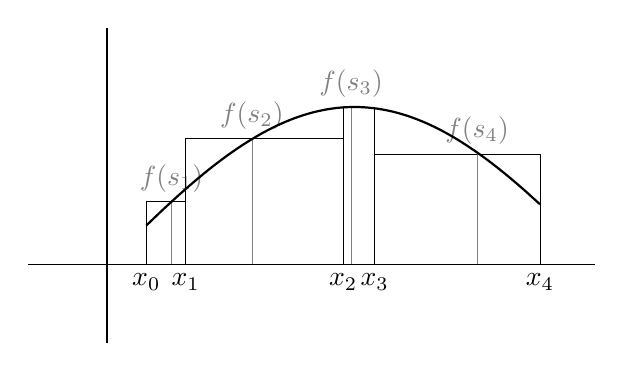
\begin{tikzpicture}[domain=0.25:2.75,scale=2]
%\draw[step=.5cm,lightgray,very thin] (-0.4,-0.4) grid (3.1,1.4);
\draw (-0.5,0) -- (3.1,0);
\draw (0,-0.5) -- (0,1.5);

\draw[black,very thin](0.25,0.2474) -- (0.25,0)  node[below]{$x_0$} ;
\draw[black,very thin](2.75,0.38166) -- (2.75,0)  node[below]{$x_4$} ;


\draw[black,very thin](0.25,0) -- (0.25,0.4);
\draw[black,very thin](0.25,0.4) -- (0.5,0.4);
\draw[black,very thin](0.5,0.4) -- (0.5,0) node[below]{$x_1$};
\draw[gray,very thin](0.41,0) -- (0.41,0.4) node[above]{$f(s_1)$};

\draw[black,very thin](0.5,0) -- (0.5,0.8);
\draw[black,very thin](0.5,0.8) -- (1.5,0.8);
\draw[black,very thin](1.5,0.8) -- (1.5,0) node[below]{$x_2$};
\draw[gray,very thin](0.92,0) -- (0.92,0.8) node[above]{$f(s_2)$};

\draw[black,very thin](1.5,0) -- (1.5,1);
\draw[black,very thin](1.7,1) -- (1.7,1);
\draw[black,very thin](1.7,1) -- (1.7,0) node[below]{$x_3$};
\draw[gray,very thin](1.55,0) -- (1.55,1) node[above]{$f(s_3)$};

\draw[black,very thin](1.7,0) -- (1.7,0.7);
\draw[black,very thin](1.7,0.7) -- (2.75,0.7);
\draw[black,very thin](2.75,0.7) -- (2.75,0);
\draw[gray,very thin](2.35,0) -- (2.35,0.7) node[above]{$f(s_4)$};

\draw[color=black,thick]   plot[smooth] (\x,{sin(\x r)});

\end{tikzpicture}
\caption{Riemann-Summe}
\label{fig:int2}
\end{figure}

In Abbildung \ref{fig:int2} ist eine Riemann-Summe mit vier Intervallen dargestellt. Die Höhe der Rechtecke über den jeweiligen Intervallen bestimmt der Funktionswert an der Stützstelle $f(s_i)$, also genau den Stellen, an denen der Graph der Funktion $f$ die waagerechten Oberkanten der Rechtecke kreuzt. Es ist zu beachten, dass die Intervalle beliebig breit sein können.

Wenn wir uns das rechte Intervall ansehen, erkennen wir, dass zwischen $x_3$ und $s_3$ das Rechteck zu tief ist. Der Graph von $f$ erhebt sich in einem Bogen darüber (diese Fläche nennen wir $g_l$), während zwischen $s_3$ und $x_4$ die Oberkante zu hoch liegt, $f$ schneidet hier eine Ecke des Rechtecks ab (diese Fläche nennen wir $g_r$). Der exakte Flächeninhalt unter dem Graphen von $f$ zwischen $x_3$ und $x_4$ ist also

\begin{equation}
F'_3 = f(s_3)(x_3-x_2)+g_l-g_r
\end{equation}

Damit unsere Rechtecke möglichst genau den Flächeninhalt bestimmen, müssen wir die $g_l$ und $g_r$ Werte so klein wie nur irgend möglich machen. Aber woher kommen diese Werte? Ganz klar liegt das daran, dass unsere Rechtecke ziemlich breit sind. Wären sie schmaler, wären die Flächen $g_l,g_r$ sehr klein. Der Fehler, den wir mit der Rechteck-Annäherung machen also auch kleiner. Wenn wir aber die Rechtecke kleiner, d.h. schmaler machen, dann müssen wir mehr Rechtecke nehmen, um die Strecke zwischen $a$ und $b$ mit Rechtecken aufzufüllen. Und dann hätten wir das Problem, dass wir nicht kontrollieren könnten, ob ein bestimmtes Intervall, zum Beispiel $[x_1,x_2]$ auch wirklich kleiner wird, oder ob nicht immer mehr Stützstellen außerhalb dieses Intervalls eingebaut würden. 

Dies wäre eine problematische Eigenschaft der Zerlegung. Um nun zu gewährleisten, dass unsere Zerlegung auch wirklich immer feiner wird, in allen Rechtecken, definieren wir uns folgende Eigenschaft der Zerlegung:

\begin{definition}\index{Feinheit einer Zerlegung}
Es sei $Z$ eine Zerlegung des Intervalls $[a,b]$. Der Wert
\begin{equation}
\mu (Z) = \max\left\{ x_{i}-x_{i-1} \middle| i=1,\dots ,N  \right\}
\end{equation}
wird als \emph{Feinheit} der Zerlegung bezeichnet.
\end{definition}

\subsection{Der Integral-Begriff}\index{Integral}

Folgende Definition geht auf Bernhard Riemann zurück:

\begin{definition}[Riemann-Integral]\index{Riemann-Integral}
Eine Funktion $f$ heißt über dem Intervall $[a,b]$ \emph{integrierbar}\index{integrierbar}, wenn die Riemann-Summen, unabhängig von Zerlegung und gewählten Stützstellen, sich einer Zahl $A$ beliebig annähern, sofern die Zerlegungen nur fein genug gewählt wird ($\mu(Z)$). Anders ausgedrückt: Zu einer Zahl $A$ und einer Zahl $\epsilon >0$ gibt es ein $\delta >0$, sodass aus $\mu(Z)<\delta$ folgt
\begin{equation}
\left| \sum_{i=1}^{N} f(s_i)\cdot (x_{i}-x_{i-1}) -A \right| < \epsilon
\end{equation}
\end{definition}

\begin{definition}
Die Zahl $A$ (wie oben) wird das \emph{bestimmte Integral} der Funktion $f$ über dem Intervall $[a,b]$ genannt und man stellt es mit dem Integralzeichen dar:
\begin{equation}
A = \int_{a}^{b} f(x) \enspace dx
\end{equation}
Dabei ist das Integralzeichen wie eine unendliche Summe über eine Zerlegung zu verstehen, während der $dx$ Operator wie die Breite eines infinitesimal schmalen Intervalls mit dem Funktionswert $f(x)$ multipliziert wird. Dies ist also nichts anderes, als unsere Rechteck-Berechnung.
\end{definition}

Neben dem \emph{Riemann-Integral} gibt es noch weitere Arten des Integralbegriffs. Eine Definition über sogenannte Ober- und Untersummen führt ebenfalls zum Riemann-Integral, während eine Definition über die Messbarkeit zum Lebesgue-Integral führt.

\section{Wichtige Integrale}

\subsection{Konstante Integrale}

Betrachten wir zunächst das Integral über der konstanten Funktion $f(x)=1$. Wir wählen eine Intervall Zerlegung $Z$ wie in Definition \ref{def:zerlegung} so, dass $\mu(Z)<\delta$ sowie Stützstellen wie oben. Dann haben wir folgende Summe zu betrachten:

\begin{equation}
\sum_{i=1}^{N} f(s_i)\cdot (x_{i}-x_{i-1}) = \sum_{i=1}^{N} 1\cdot (x_{i}-x_{i-1})
\end{equation}
denn der Funktionswert ist überall gleich $1$. Damit ist die Summe eine sogenannte Teleskop-Summe, das heißt, ihre inneren Glieder kürzen sich alle weg und es bleiben nur der erste und letzte Term übrig.
\begin{equation}
\begin{split}
\sum_{i=1}^{N} (x_{i}-x_{i-1}) &=(x_1-x_0)+(x_2-x_1)+(x_3-x_2)+\dots +(x_N-x_{N-1}) \\
&= x_N\underbrace{-x_{N-1}+x_{N-1}}_{=0} \underbrace{-x_{N-2}+x_{N-2}}_{=0}+ \dots \underbrace{-x_2+x_2}_{=0} \underbrace{-x_1+x_1}_{=0}-x_0 \\
&= x_N-x_0\\
&=b-a
\end{split}
\end{equation}
Das gilt für alle beliebigen Zerlegungen. Wir benutzen die Definition des Integrals: Zu jedem $\epsilon$ gibt es ein $\delta$, sodass aus $\mu(Z)<\delta$ folgt
\begin{equation}\label{eq:baA}
\begin{split}
\left| \sum_{i=1}^{N} f(s_i)(x_{i}-x_{i-1}) -A \right| &= \left| \sum_{i=1}^{N} (x_{i}-x_{i-1}) -A \right| \\ 
&=\left| b-a - A \right| < \epsilon
\end{split}
\end{equation}
Wenn Ungleichung (\ref{eq:baA}) korrekt ist -- d.h. für jedes beliebig kleine $\epsilon$ gilt 
\begin{equation}
|b-a-A|<\epsilon,
\end{equation}
dann muss $A=b-a$ sein. Sprich:
\begin{equation}
\int_a^b 1 \enspace dx = (b-a)
\end{equation}

Mit dem selben Argument kann man folgern, dass für eine konstante Zahl $c\in \mathbb{R}$ gilt:

\begin{equation}
\int_a^b c \enspace dx = c\cdot(b-a)
\end{equation}
denn wir können den Faktor $c$ aus der Summe ausklammern:
\begin{equation}
\begin{split}
\left| \sum_{i=1}^{N} f(s_i)(x_{i}-x_{i-1}) -A \right| &= \left| \sum_{i=1}^{N} c\cdot (x_{i}-x_{i-1}) -A \right| \\ 
&=\left| c\cdot \sum_{i=1}^{N} (x_{i}-x_{i-1}) -A \right|\\
&=\left| c\cdot (b-a) -A \right| < \epsilon
\end{split}
\end{equation}

\subsection{Lineare Integrale}

Betrachten wir hier nun $f(x) = c\cdot x$ mit $c\in \mathbb{R}$ einem konstanten Wert. 

\begin{equation}
\begin{split}
\left| \sum_{i=1}^{N} f(s_i)(x_{i}-x_{i-1}) -A \right| &= \left| \sum_{i=1}^{N} c\cdot s_i \cdot (x_{i}-x_{i-1}) -A \right| \\ 
&=\left|  c\cdot \sum_{i=1}^{N}s_i \cdot (x_{i}-x_{i-1}) -A \right|
\end{split}
\end{equation}
Die Stützstellen sind so gewählt, dass
\begin{equation}
x_{i-1} \le s_i \le x_{i}
\end{equation}
Jedoch gibt es bei linearen Funktionen eine besondere Wahl für die Stützstellen: Und zwar genau in der Mitte des Intervalls: $s_i = \frac{1}{2}(x_{i}+x_{i-1})$. Dann gleichen sich die Fehler ober- und unterhalb der Funktion aus. Es ist zwar richtig, dass wir beliebige Stützstellen zulassen wollen, aber in diesem Fall können wir direkt mit dem korrekten Integral auf den Intervallen arbeiten, was uns die Sache erheblich erleichtert. Wir verwenden die Stützstellen in der Mitte des Intervalls und wenden die dritte Binomische Formel (\ref{eq:binom3}) an:
\begin{equation}
\begin{split}
\left|  c\cdot \sum_{i=1}^{N}s_i \cdot (x_{i}-x_{i-1}) -A \right| &= \left|  c\cdot \sum_{i=1}^{N} \frac{1}{2}(x_{i}+x_{i-1}) \cdot (x_{i}-x_{i-1}) -A \right|\\
&=\left|  c\cdot \frac{1}{2} \cdot \sum_{i=1}^{N} (x_{i}^2-x_{i-1}^2) -A \right|, \text{ wieder eine Teleskopsumme}\\
&=\left|  c\cdot \frac{1}{2} \cdot (b^2-a^2) -A \right| < \epsilon
\end{split}
\end{equation}
Und auch hier gilt wieder, dass sich der letzte konstante Ausdruck nur dann kleiner als jedes beliebige $\epsilon$ machen lässt, wenn gilt
\begin{equation}
A = c\cdot \frac{1}{2} \cdot (b^2-a^2)
\end{equation}
und somit
\begin{equation}
\int_a^b c\cdot x \enspace dx = c\cdot \frac{1}{2} \cdot (b^2-a^2)
\end{equation}


\section{Kriterien der Integrierbarkeit}
TODO 

\section{Das unbestimmte Integral}
TODO

\section{Hauptsatz der Differential- und Integralrechnung}

Bevor wir zum eigentlichen Hauptsatz kommen, brauchen wir zwei Zwischenergebnisse. Zum einen untersuchen wir die Möglichkeit, das Integral durch obere und untere Schranken der Funktion $f$ abzuschätzen. Und weiter werden wir den Mittelwertsatz kennen lernen, der uns die Möglichkeit eröffnet, das Integral einer Funktion durch einen speziellen Funktionswert darzustellen. 

\begin{satz}\label{satz:mittel}
Es sei $f$ eine über dem Intervall $[a,b]$ (Riemann-) integrierbare Funktion. Dann gibt es Zahlen $f_{\sup}, f_{\inf} \in \mathbb{R}$ der folgenden Art:

\begin{equation}
f_{\inf}\cdot (b-a) \le \int_{a}^{b} f(x) \enspace dx \le f_{\sup} \cdot (b-a)
\end{equation}
\end{satz}
\begin{proof}
Der Beweis ist trivial, denn mit Auswahl des Infimums und des Supremums wird der Integrand zu einer Konstanten, die aus dem Integral herausgezogen werden kann. Denn wir wissen, dass für eine Konstante $c$ folgendes gilt:
\begin{equation}
\int_a^b c \enspace dx = c\cdot \int_a^b 1 \enspace dx = c\cdot \int_a^b dx = c\cdot(b-a)
\end{equation}
Also ist
\begin{equation}
\begin{split}
\int_a^b f(x)\enspace dx &\ge \int_a^b \underbrace{\inf_{\xi \in [a,b] } f(\xi)}_{\text{konstant}} \enspace dx \\
 &= \inf_{\xi \in [a,b] } f(\xi) \cdot (b-a) \\
 &= f_{\inf}\cdot (b-a)
\end{split}
\end{equation}
und weiter
\begin{equation}
\begin{split}
\int_a^b f(x)\enspace dx &\le \int_a^b \underbrace{\sup_{\xi \in [a,b] } f(\xi)}_{\text{konstant}} \enspace dx \\
 &= \sup_{\xi \in [a,b] } f(\xi) \cdot (b-a) \\
 &= f_{\sup}\cdot (b-a)
\end{split}
\end{equation}
somit folgt unsere Behauptung.
\end{proof}


\begin{satz}[Mittelwertsatz der Integralrechnung]
Es sei $f$ eine integrierbare Funktion über dem Interval $[a,b]$. Dann gibt es ein $\xi \in [a,b]$, sodass 
\begin{equation}
\int_a^b f(x) \enspace dx = f(\xi) \cdot (b-a)
\end{equation}
\end{satz}
\begin{proof}
Im vorher gehenden Satz \ref{satz:mittel} hatten wir gesehen, dass für $f$ gilt
\begin{equation}
f_{\inf}\cdot (b-a) \le \int_{a}^{b} f(x) \enspace dx \le f_{\sup} \cdot (b-a)
\end{equation}
Es gibt also ein $\eta \in [f_{\inf},f_{\sup}]$, sodass 
\begin{equation}
\int_{a}^{b} f(x) \enspace dx = \eta \cdot (b-a)
\end{equation}
Aus dem Zwischenwertsatz (\ref{satz:zwischen}) folgt daraus dann, dass es ein $\xi \in [a,b]$ gibt mit 
\begin{equation}
f(\xi) = \eta
\end{equation}
Und somit folgt die Behauptung
\begin{equation}
\int_a^b f(x) \enspace dx = f(\xi) \cdot (b-a)
\end{equation}
\end{proof}

\begin{satz}[Hauptsatz der Differential- und Integralrechnung]
Es sei $f$ eine stetige und (Riemann-) integrierbare Funktion über dem Intervall $[a,b]$. Weiter ist eine \emph{Integralfunktion} (oder auch \emph{Stammfunktion}) auf dem Intervall definiert
\begin{equation}
F(z_0,z) = \int_{z_0}^z f(x) \enspace dx + c
\end{equation}
für alle $z_0 \in [a,b]$ und einer beliebigen Konstante $c\in \mathbb{R}$. Dann sind folgende Aussagen richtig:

\begin{enumerate}
\item $F(z_0,z)$ ist differenzierbar und es gilt $F'(z_0,z) = f(z)$.
\item Für das bestimmte Integral gilt \begin{equation}
\int_a^b f(x) \enspace dx = F(a,b)-F(a,a)
\end{equation}
\end{enumerate}
\end{satz}
\begin{proof}
Zunächst betrachten wir den Differenzenquotienten von $F$
\begin{equation}
\begin{split}
\lim_{h\rightarrow 0} \frac{F(z_0,z+h)-F(z_0,z)}{h} &= \lim_{h\rightarrow 0} \frac{\int_{z_0}^{z+h} f(x)\enspace dx+c - \int_{z_0}^{z} f(x)\enspace dx-c}{h} \\
&= \lim_{h\rightarrow 0}\frac{1}{h} \int_{z}^{z+h} f(x)\enspace dx \\
&= \lim_{h\rightarrow 0}\frac{1}{h} f(\xi)\cdot (z+h-z)\enspace dx, \text{ mit dem Mittelwertsatz} \\
&= f(z), \text{ da }\xi \rightarrow z\text{, für }h\rightarrow 0
\end{split}
\end{equation}
Das bedeutet, die Ableitung von $F$ existiert und ist gerade $F'(z_0,z)=f(z)$. Der zweite Teil des Beweises wird durch einfaches Einsetzen erreicht. Wir setzen $z_0 = a$ und für diesen Fall lassen wir das erste Argument von $F$ meistens weg. Dann ist $F(a,a)=F(a)=c$ und
\begin{equation*}
F(a,b)=F(b) = \int_a^b f(x) \enspace dx +c
\end{equation*}
daher ist
\begin{equation}
\int_a^b f(x) \enspace dx = F(b)-F(a)
\end{equation}
\end{proof}

\section{Stammfunktion}

TODO

\section{Anwendungen}

\subsection{Substitution des Funktionswertes}

Ein Integral berechnet, wie wir gelernt haben, den Flächeninhalt unter einer Funktion. Hierfür werden unendlich viele, unendlich dünne Rechtecke aufsummiert. Ein unendlich dünnes Rechteck ist aber nichts anderes als ein Strich. Was würde passieren, wenn wir den Strich zum Beispiel durch einen Kreis ersetzen? Der Kreisinhalt ist $\pi r^2$. Anstatt nun Striche zu summieren, integrieren wir über den Flächeninhalt von Kreisen. Dies entspricht der Berechnung eines Volumenkörpers, dessen Rand der Funktion $f$ entspricht, und der in jeder "`Scheibe"' kreisförmigen Durchschnitt hat. Also gerade so, als ob der Graph der Funktion $f$ um die $x$-Achse rotieren würde. Einen solchen Körper bezeichnet man daher als \emph{Rotationskörper} und sein Volumen wird wie folgt berechnet:

\begin{equation}
V_{\text{rot}}(f,a,b) = \int_a^b \pi f(x)^2 \enspace dx=  \pi \int_a^b f(x)^2 \enspace dx
\end{equation}

TODO

\section{Aufgaben}